\chapter{Distributions of one Variable}


\section{Characterizing a Distribution}

\subsection{ Distribution Center }
\subsubsection{ Mean } \index{general}{mean}
By default, when we talk about the \emph{mean value} we mean the \emph{arithmetic mean} $\bar{x}$:

\begin{equation}
  \bar{x} = \frac{{\sum\limits_{i = 1}^n {{x_i}} }}{n}
\end{equation}

\subsubsection{ Median } \index{general}{median}
The \emph{median} is that value that comes half-way when the data are ranked in order.
In contrast to the mean, it is not affected by outlying data points.

\subsubsection{ Mode } \index{general}{mode}
The \emph{mode} value is the most frequently occurring value in a distribution.

\subsubsection{ Geometric Mean }\index{general}{geometric mean}
In some situations the \emph{geometric mean} can be useful to describe the location of a distribution. It is usually close to the median, and can be calculated via the arithmetic mean of the log of the values.

\subsection{ Quantifying Variability }\label{sec:centiles}

\subsubsection{ Range }\index{general}{range}
This one is fairly easy: it is the difference between the highest and the lowest data value.
The only thing that you have to watch out for: after you have acquired your data, you have to check for \emph{outliers}, i.e. data points with a value much higher or lower than the rest of the data. Often, such points are caused by errors in the selection of the sample or in the measurement procedure. There are a number of tests to check for outliers. One of them is to check for data which lie more than 1.5*\emph{inter-quartile-range} (IQR) above or below the first/third quartile (see below).


\subsubsection{ Centiles }\index{general}{centiles}\index{general}{percentiles}
The \emph{Cumulative distribution function (CDF) } \index{general}{cumulative distribution function} tells you for each value which percentage of the data has a lower value (Figure \ref{fig:CDF}). The value below which a given percentage of the values occur is called \emph{centile} or \emph{percentile}, and corresponds to a value with a specified cumulative frequency.

For example, when you look for the data range which includes 95\% of the data, you have to find the $2.5^{th}$ and the $97.5^{th}$ percentile of your sample distribution.

The 50th percentile is the \emph{median}.

Also important are the \emph{quartiles}, i.e. the 25th and the 75th percentile. The difference between them is sometimes referred to as \emph{inter-quartile range (IQR)}\index{general}{IQR}.

Median, upper and lower quartile are used for the data display in box plots (Fig.\ref{fig:Boxplot}).

\begin{figure}[ht]
  \centering
  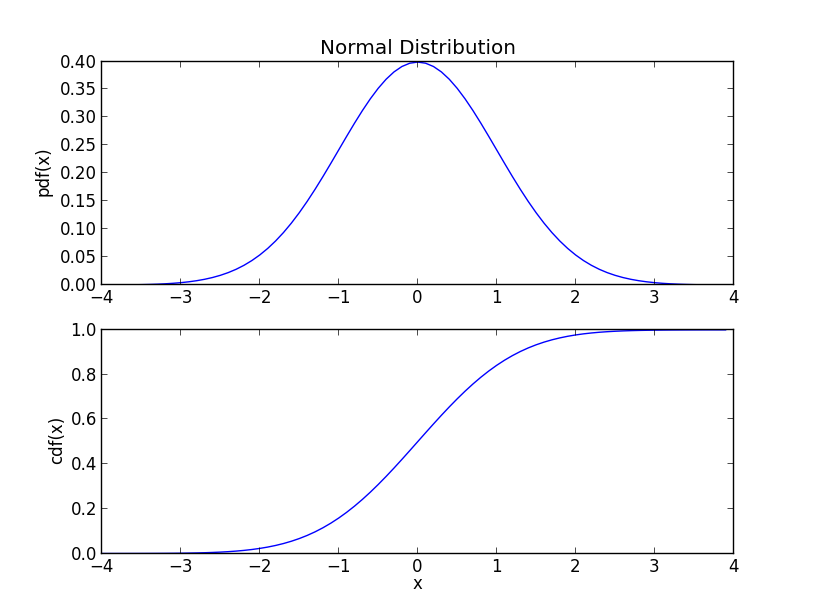
\includegraphics[width=0.5\textwidth]{../Images/NormalDist_PDF_CDF.png}\\
  \caption{\emph{Probability distribution function} (top) and \emph{Cumulative distribution function} (bottom) of a normal distribution.}\label{fig:CDF}
\end{figure}


\subsubsection{ Standard Deviation and Variance }
The \emph{variance} (SD) of a distribution is defined as

\begin{equation}\label{eq_variance} \index{general}{variance}
  var = \frac{{\sum\limits_{i = 1}^n {({x_i-\bar{x}})^2} }}{n-1}
\end{equation}

Note that we divide by \emph{n-1} rather than the more obvious n: dividing by $n$ gives the variance of the observations around the sample mean, but we virtually always consider our data as a sample from some larger population and wish to use the sample data to estimate the variability in the population. Dividing by $n-1$ gives us a better estimate of the population variance.

The \emph{standard deviation} \index{general}{standard deviation} is simply given by the square root of the variance:

\begin{equation}
  s = \sqrt{var}
\end{equation}

In statistics it is often common to denote the population standard deviation with $\sigma$, and the sample standard deviation with $s$.

Watch out: in Python, by default the variance is calculated for "n". You have to set "ddof=1" to obtain the variance for "n-1":

\begin{lstlisting}
    In[19]: data = arange(7,14)

    In[20]: std(data, ddof=0)
    Out[20]: 2.0

    In[21]: std(data, ddof=1)
    Out[21]: 2.1602468994692865
\end{lstlisting}

\subsubsection{ Standard Error } \index{general}{standard error}
While the standard deviation is a good measure for the distribution of your values, often you are more interested in the distribution of the mean value. For example, when you measure the response to a new medication, you might be interested in how well you can characterize this response, i.e. is how well you know the mean value. This measure is called the \emph{standard error of the mean}, or sometimes just the \emph{standard error}. In a single sample from a population with a standard deviation of $\sigma$ the variance of the sampling distribution of the mean is $\sigma^2/n$, and so the standard error of the mean is $\sigma/\sqrt{n}$.

\subsubsection{ Skewness }\index{general}{skewness}
Distributions are \emph{skewed} if they depart from symmetry. For example, if you have a measurement that cannot be negative, which is usually the case, then we can infer that the data have a skewed distribution if the standard deviation is more than half the mean. Such an asymmetry is referred to as \emph{positive skewness}. The opposite, negative skewness, is rare.

\subsubsection{ Central Limit Theorem }\index{general}{central limit theorem}
The central limit theorem states that for identically distributed independent random variables (also referred to as \emph{random variates})\index{general}{variate}, the mean of a sufficiently large number of these variables will be approximately normally distributed.

%(Lecture 5)

\section{Distribution Functions}

The variable for a standardized distribution function is often called \emph{statistic}\index{general}{statistic}. So you often find expressions like "the z-statistic" (for the normal distribution function), the "t-statistic" (for the t-distribution) or the "F-statistic" (for the F-distribution).

  \subsection{Probability and Samples}

  \subsection{Normal Distribution} \label{sec:normalDistribution}\index{general}{distributions!normal}

The \emph{Normal distribution} or \emph{Gaussian distribution} is by far the most important of all the distribution functions. This is due to the fact that the mean values of \emph{all} distribution functions approximate a normal distribution for large enough sample numbers.
Mathematically, the normal distribution is characterized by a mean value $\mu$, and a standard deviation $\sigma$:

\begin{equation}\label{eq_normal}
     f_{\mu,\sigma} (x) = \frac{1}{\sigma \sqrt{2 \pi}} e^{-( x - \mu )^2 /2 \sigma^2}
\end{equation}
where $ - \infty < x < \infty $, and $f_{\mu,\sigma}$ is the \emph{probability density function (PDF)} \index{general}{probability density function}.

\begin{figure}
  \centering
  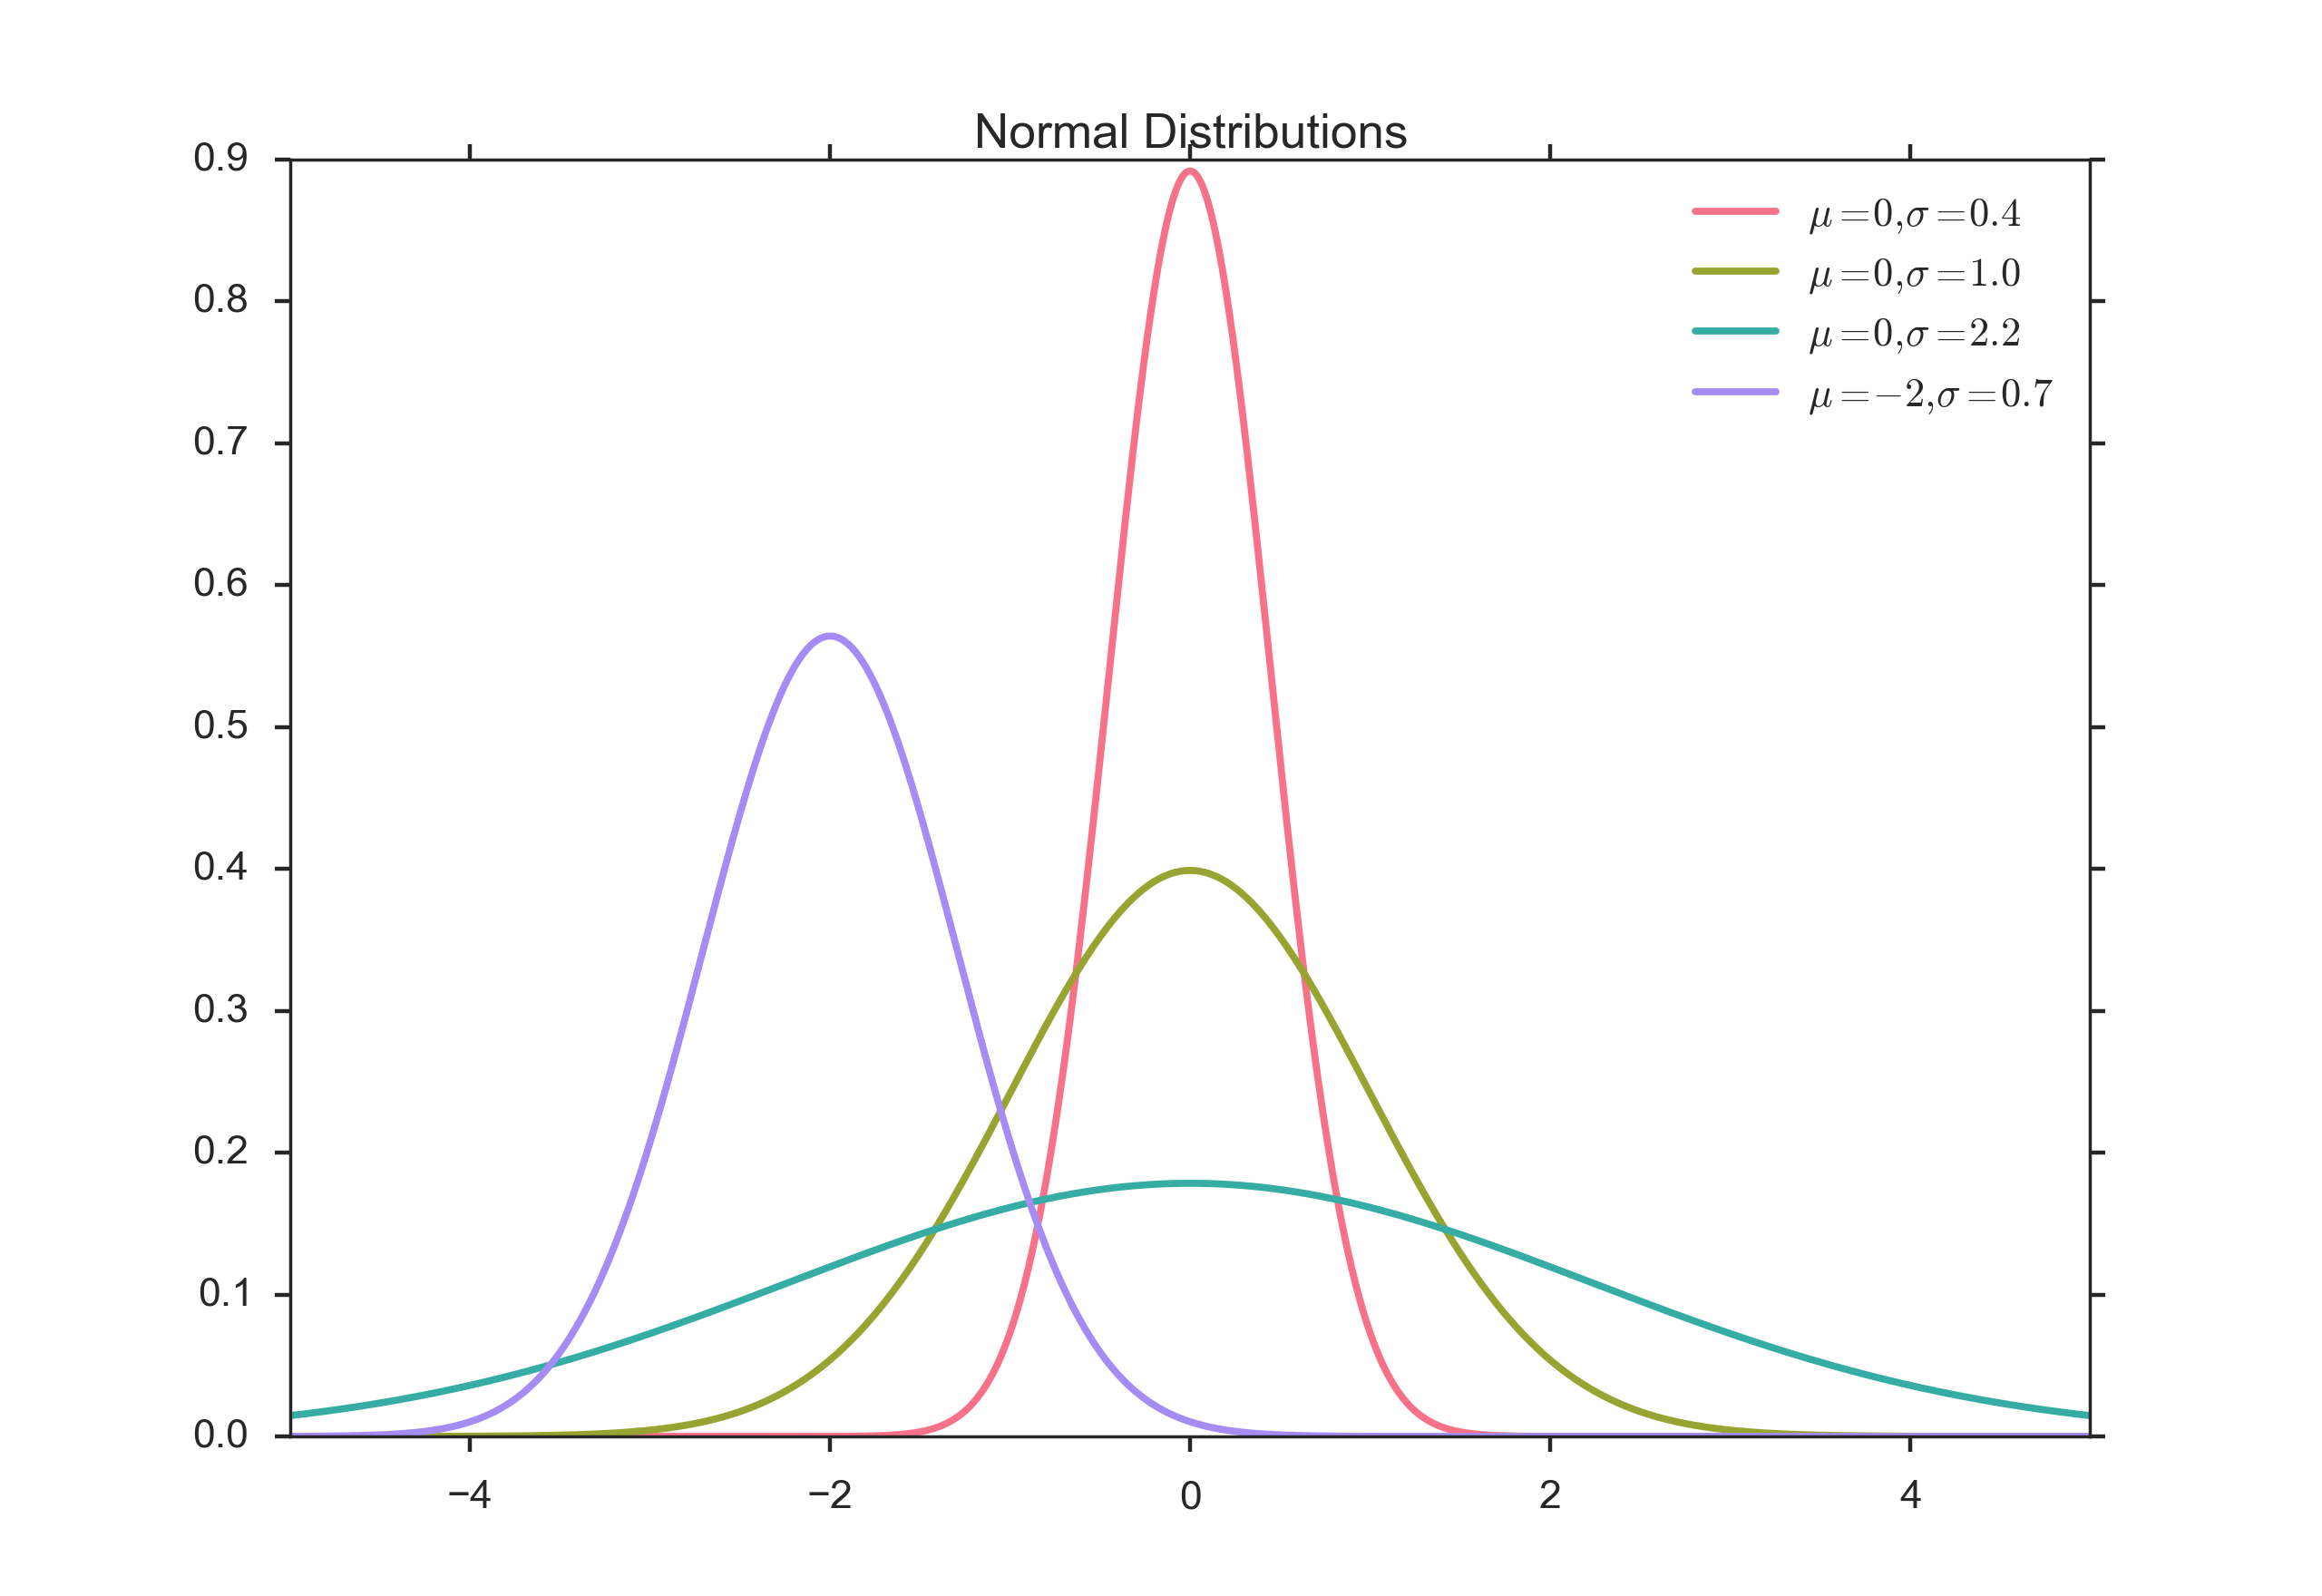
\includegraphics[width=0.75\textwidth]{../Images/Normal_Distribution_PDF.png}\\
  \caption{Normal Distribution}\label{fig:normal}
\end{figure}

For smaller sample numbers, the sample distribution can show quite a bit of variability. For example, look at 25 distributions generated by sampling 100 numbers from a normal distribution (Fig. \ref{fig:MultipleNormal})

\begin{figure}[h]
  \centering
  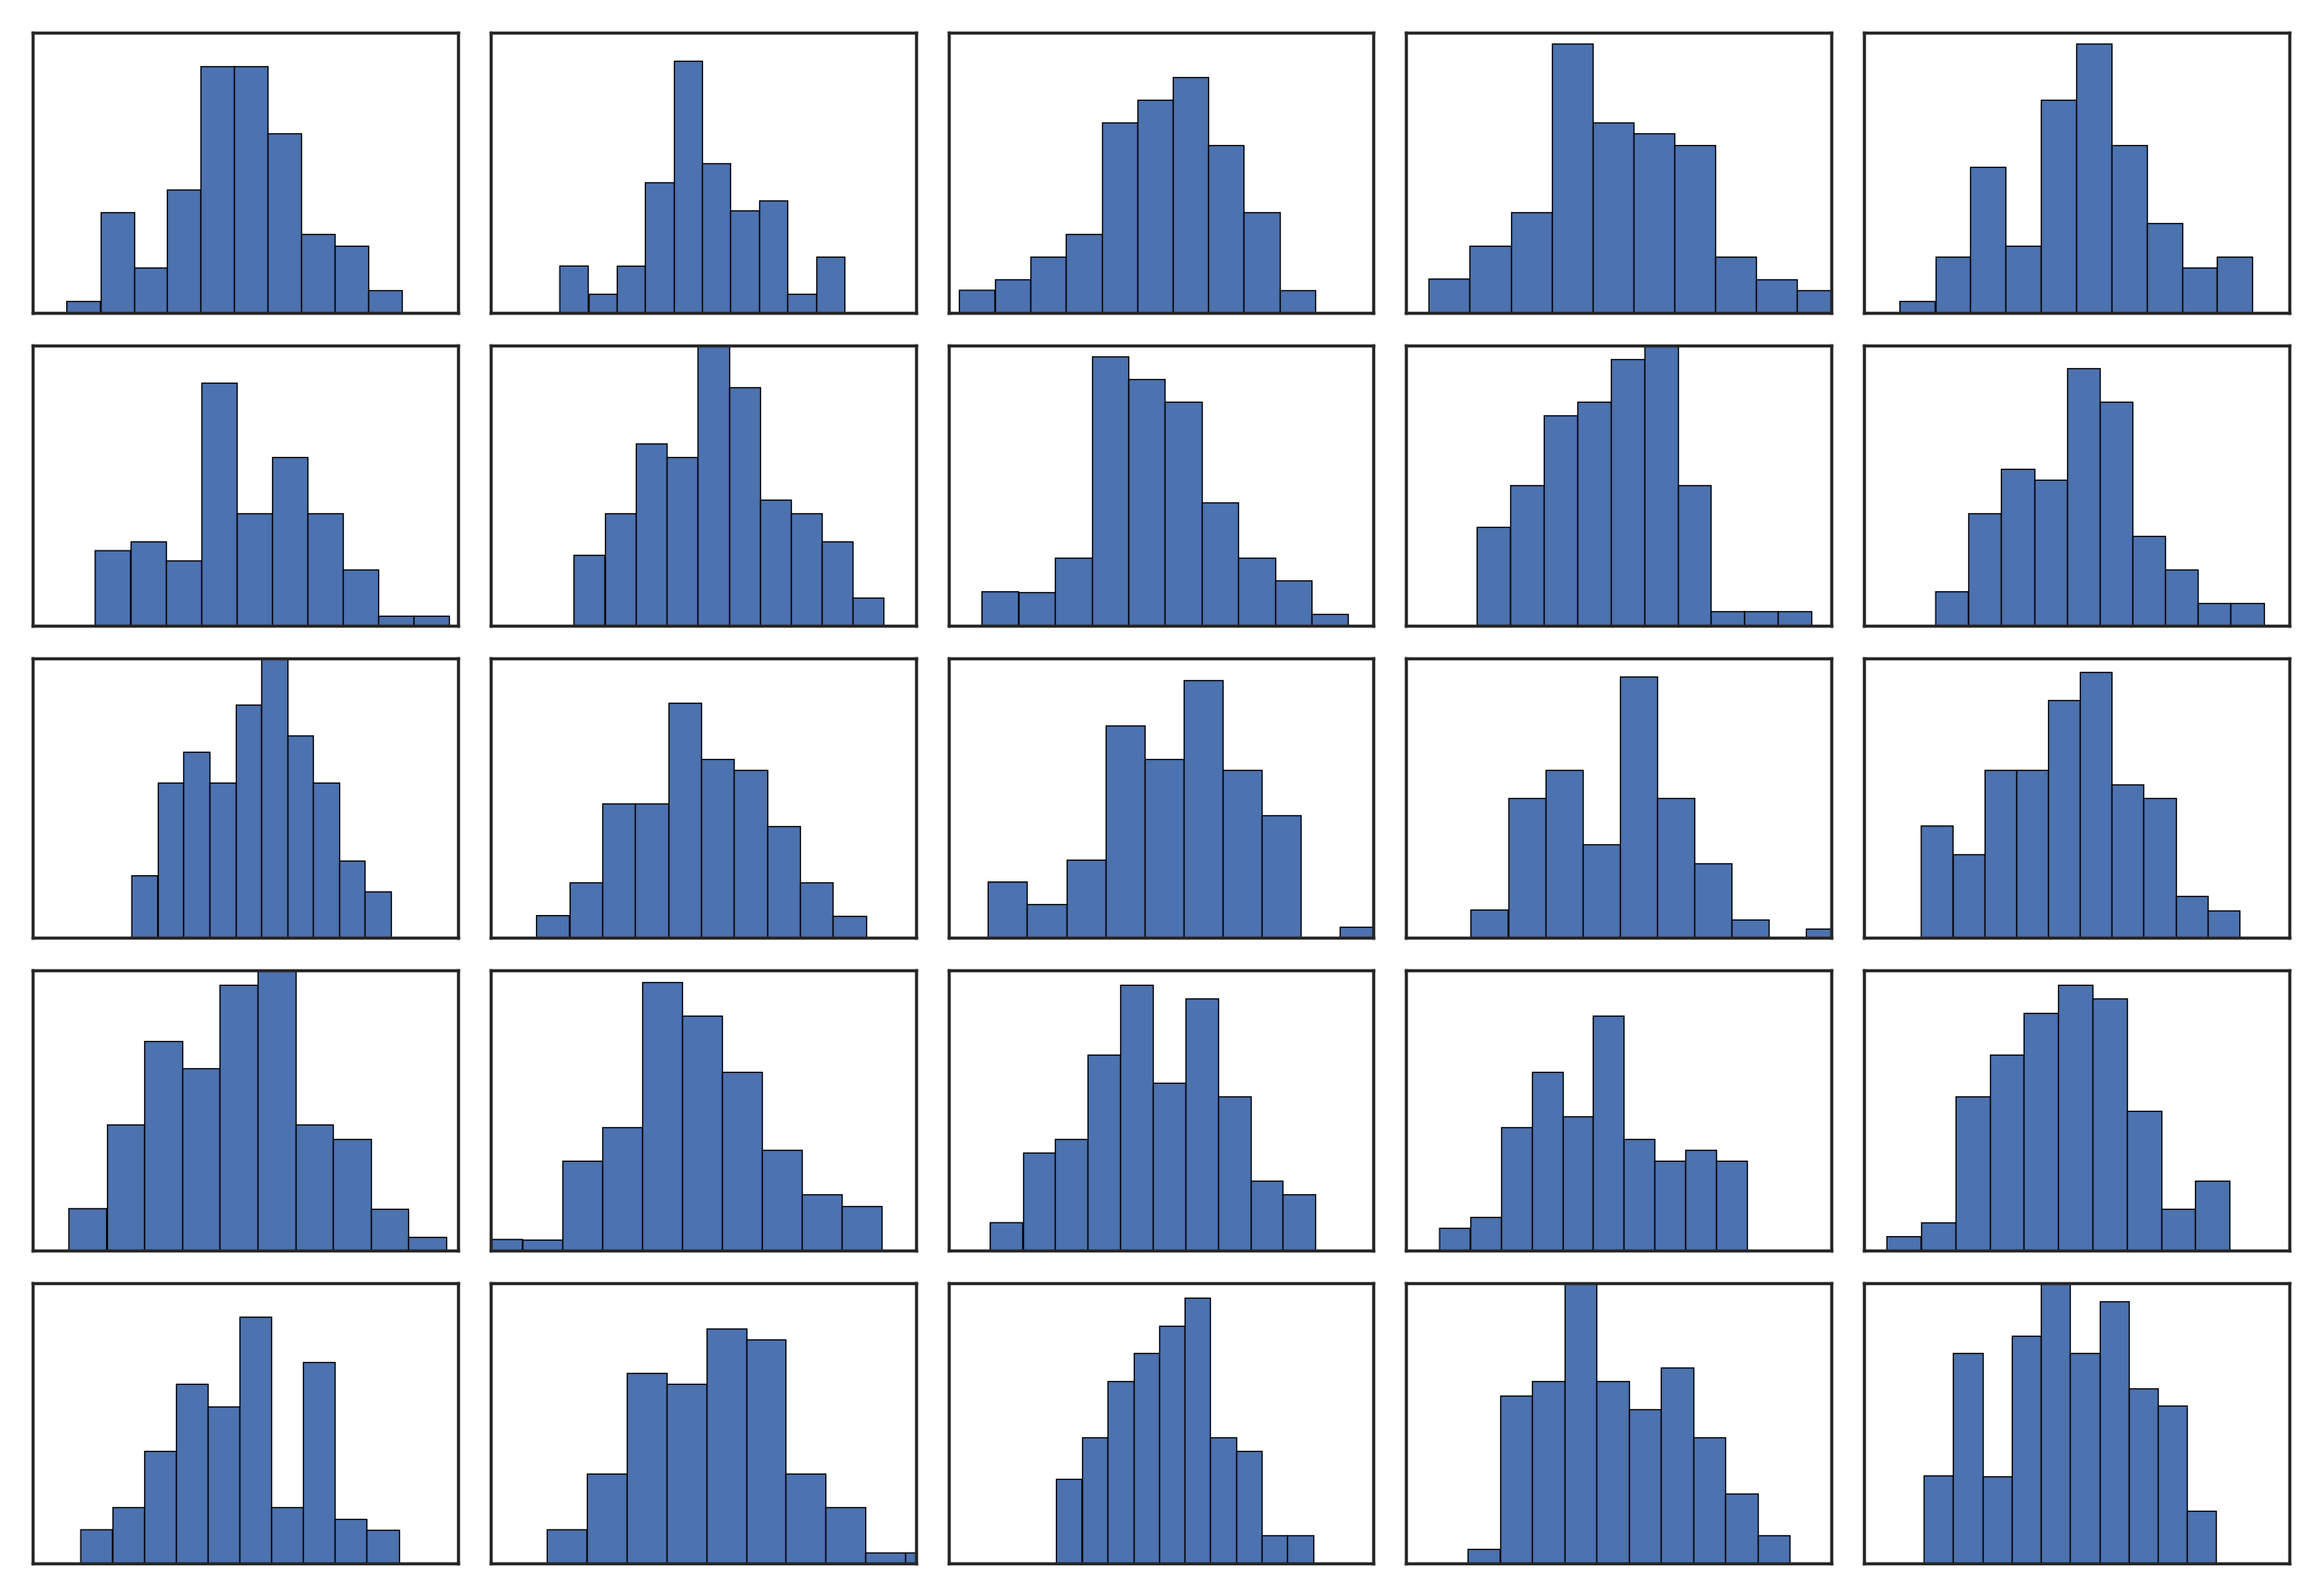
\includegraphics[width=0.75\textwidth]{../Images/Normal_MultHist.png}\\
  \caption{25 randomly generated normal distributions of 100 points.}\label{fig:MultipleNormal}
\end{figure}

Some examples of applications are:

\begin{itemize}
\item{}If the average man is 175 cm tall with a variance of 6 cm, what is the probability that a man found at random will be 183 cm tall?
\item{}If the average man is 175 cm tall with a variance of 6 cm and the average woman is 168 cm tall with a variance of 3 cm, what is the probability that the average man from a given sample will be shorter than the average woman from a given sample?
\item{}If cans are assumed to have a variance of 4 grams, what does the average weight need to be in order to ensure that the 99\% of all cans have a weight of at least 250 grams?

\end{itemize}

The normal distribution with parameters $\mu$ and $\sigma$ is denoted as {$N(\mu,\sigma)$}. If the \emph{random variate (rv)} {\itshape X} is normally distributed with expectation $\mu$ and standard deviation $\sigma$, one denotes: {$\,X \sim N(\mu,\sigma)$} or $\,X \in N(\mu,\sigma)$.

\begin{table}
  \centering
  \begin{tabular}{c c c}
    \hline
     & \multicolumn{2}{ c } {Probability of being} \\
    Range & within range & outside range \\
    \hline
    % after \\: \hline or \cline{col1-col2} \cline{col3-col4} ...
    mean $\pm$ 1SD & 0.683 & .317 \\
    mean $\pm$ 2SD & 0.954 & 0.046 \\
    mean $\pm$ 3SD & 0.9973 & 0.0027 \\
    \hline
  \end{tabular}
  \caption{Tails of a normal distribution.}
\end{table}


Figure \ref{fig:DistributionUtilities} shows a number of functions are commonly used to select appropriate points from the normal distribution function:

\begin{itemize}
  \item \emph{Probability density function (PDF)}: note that to obtain the probability for the variable appearing in a certain interval, you have to \emph{integrate} the PDF over that range.
  \item \emph{Cumulative distribution function (CDF)}: gives the probability of obtaining a value smaller than the given value
  \item \emph{Survival function (SF)}: 1-CDF
  \item \emph{Percentile point function (PPF)}: the inverse of the CDF. Answers the question "Given a certain probability, what is the corresponding value for the CDF?"
  \item \emph{Inverse survival function (ISF)}: the name says it all.
\end{itemize}

\begin{figure}[h]
  \centering
  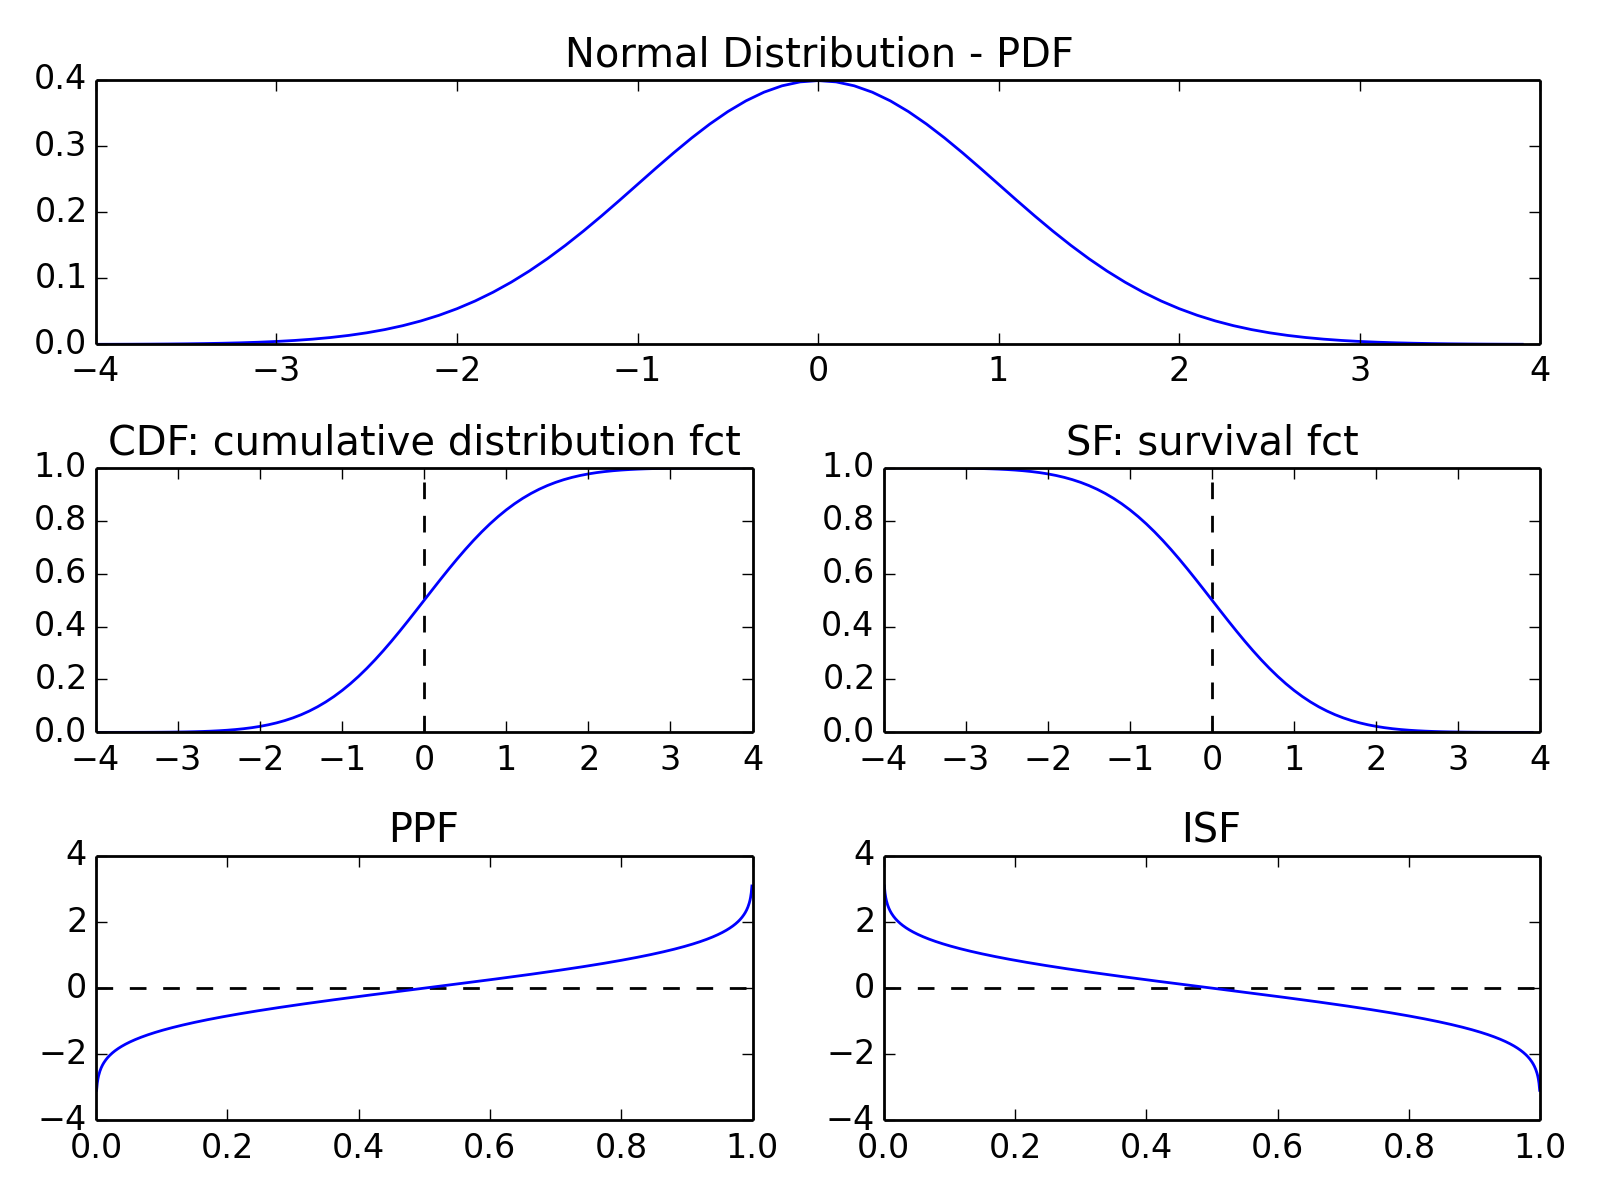
\includegraphics[width=0.75\textwidth]{../Images/DistributionFunctions.png}\\
  \caption{Utility functions for continuous distributions, here for the normal distribution.}\label{fig:DistributionUtilities}
\end{figure}

%(Lecture 6)

\subsection{Other Continuous Distributions}\label{sec:ContinuousDistributions} \index{general}{distributions!continuous}

\subsubsection{t Distribution}\index{general}{distributions!t-distribution}
For a small number of samples (ca.$<10$) from a normal distribution, the distribution of the mean deviates slightly from the normal distribution. The reason is that the sample mean does not coincide exactly with the population mean. This modified distribution is the \emph{t-distribution}, and converges for larger values towards the normal distribution (Fig. \ref{fig:t}).

\begin{figure}
  \centering
  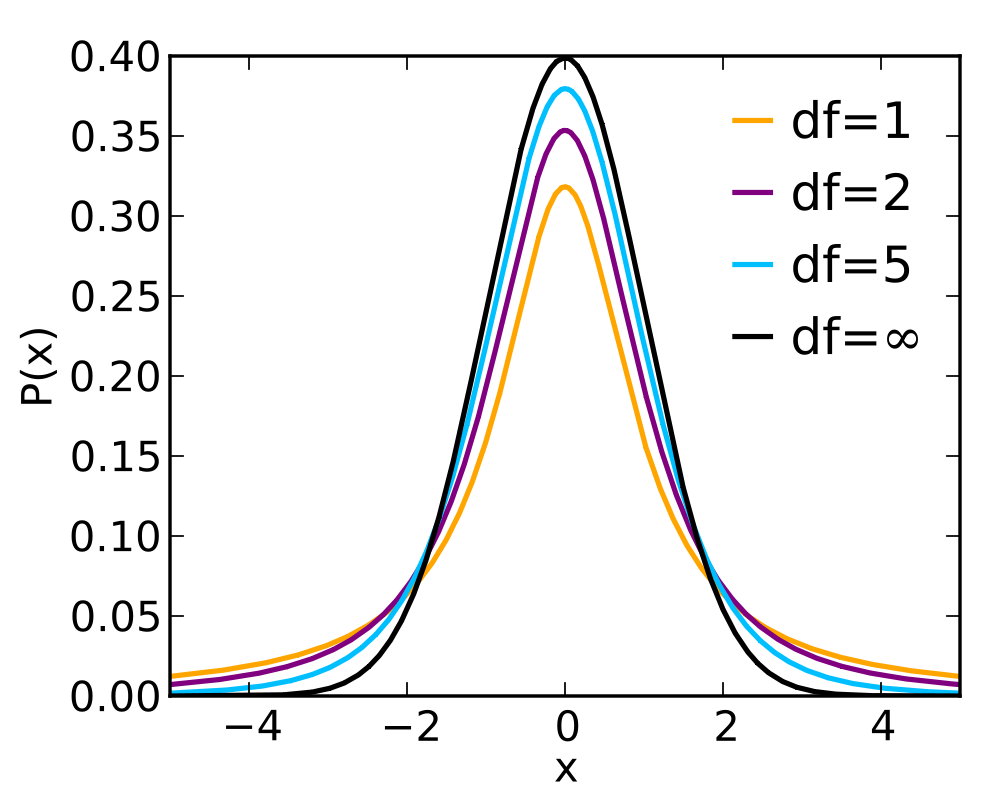
\includegraphics[width=0.5\textwidth]{../Images/Student_t_pdf.png}\\
  \caption{t Distribution}\label{fig:t}
\end{figure}


\subsubsection{Chi-square Distribution}\index{general}{distributions!chi square}

The \emph{Chi-square distribution} is related to normal distribution in a simple way: If a random variable $X$ has a normal distribution ($X \in N(0,1)$), then $X^2$ has a chi-square distribution, with one degree of freedom ($X^2 \in \chi_{1}^2$). The sum squares of $n$ independent and standard normal random variables has a chi-square distribution with $n$ degrees of freedom:

\begin{equation}
    \sum\limits_{i = 1}^n {X_i^2} \in \chi_{n}^2
\end{equation}


\begin{figure}
  \centering
  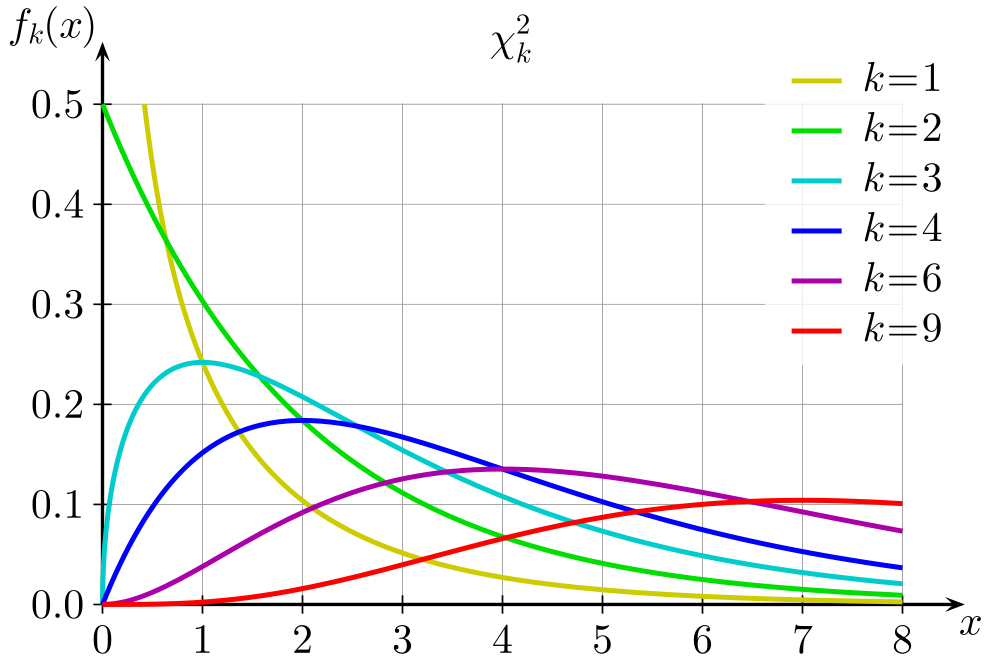
\includegraphics[width=0.5\textwidth]{../Images/ChiSquare_pdf.png}\\
  \caption{Chi-square Distribution}
\end{figure}


\subsubsection{F Distribution}\index{general}{distributions!F distribution}
Named after Sir Ronald Fisher, who developed the F distribution for use in determining critical values in ANOVAs (\emph{ANalysis Of VAriance}).  The cutoff values in an F table are found using three variables:

\begin{itemize}
  \item ANOVA numerator degrees of freedom
  \item ANOVA denominator degrees of freedom
  \item significance level
\end{itemize}

ANOVA compares the size of the variance between two different samples. This is done by dividing the larger variance over the smaller variance. The formula for the resulting \emph{F statistic} is:

\begin{equation}
    F(r_1, r_2) = \frac{\chi_{r1} ^2 /r_1}{\chi_{r2} ^2 /r_2}
\end{equation}

where $\chi_{r1}^2$ and $\chi_{r2}^2$ are the chi-square statistics of sample one and two respectively, and $r_1$ and $r_2$ are their degrees of freedom, i.e. the number of observations.

\paragraph{F-Test of Equality of Variances}
One example could be if you want to compare apples that look alike but are from different trees and have different sizes. If you want to investigate whether they have the same variance of the weight on average, you have to calculate

\begin{equation}
  F = \frac{S_x^2}{S_y^2}
\end{equation}

where $S_x$ ist he sample standard deviation of the first batch of apples, and $S_y$ the sample standard deviation for the second batch of apples.

There are three apples from the first tree that weigh 110, 121 and 143 grams respectively, and four from the other which weigh 88, 93, 105 and 124 grams respectively. The F statistic is $F 1.05$, and has $n-1$ and $m-1$ degrees of freedom, where $n$ and $m$ are the number of apples in each batch. The code sample below shots what the F statistic is close to the center of the distribution, so we cannot reject the hypthesis that the two batches have the same variance.

\begin{lstlisting}
  In [1]:  apples1 = array([110, 121, 143])
  In [2]:  apples2 = array([88, 93, 105, 124])
  In [3]:  fval = std(apples1, ddof=1)/std(apples2, ddof=1)
  In [4]:  fd = stats.distributions.f(3,4)
  In [5]:fd.cdf(fval)
  Out[27]: 0.537640478466751
\end{lstlisting}

\begin{figure}
  \centering
  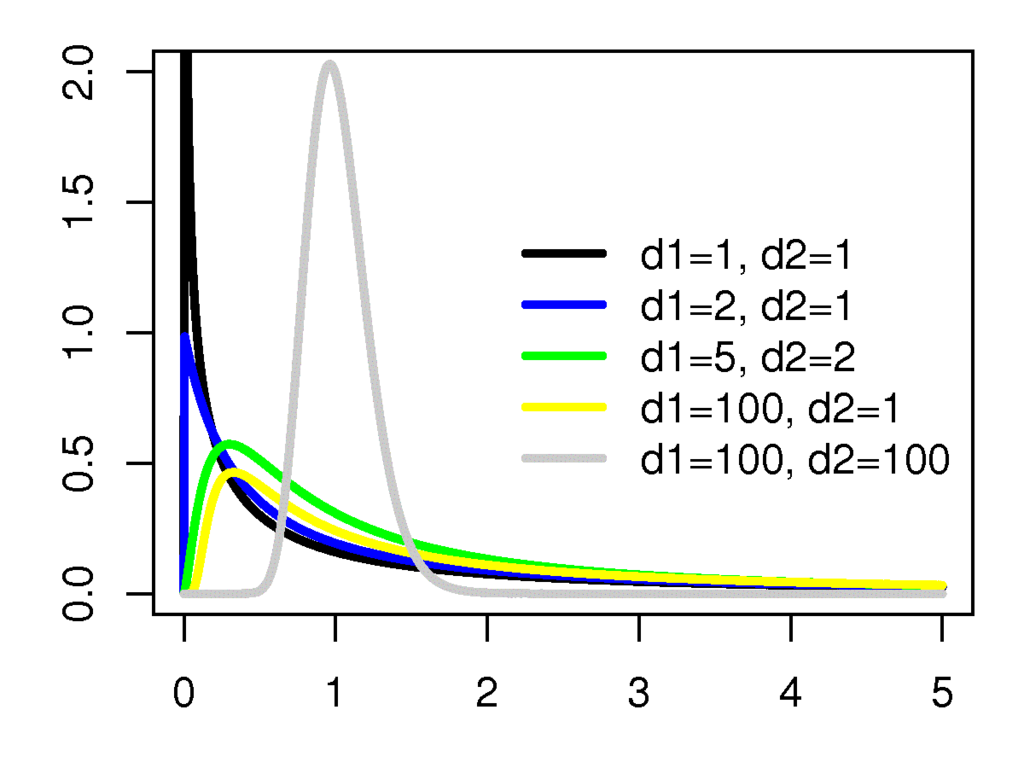
\includegraphics[width=0.5\textwidth]{../Images/F_distributionPDF.png}\\
  \caption{F Distribution}
\end{figure}


\subsubsection{Lognormal Distribution}\index{general}{distributions!lognormal}

In some circumstances a set of data with a positively skewed distribution can be transformed into a symmetric distribution by taking logarithms. Taking logs of data with a skewed distribution will often give a distribution that is near to normal (see Figure \ref{fig:lognormal}).

\begin{figure}
\centering
\begin{subfigure}{.5\textwidth}
  \centering
  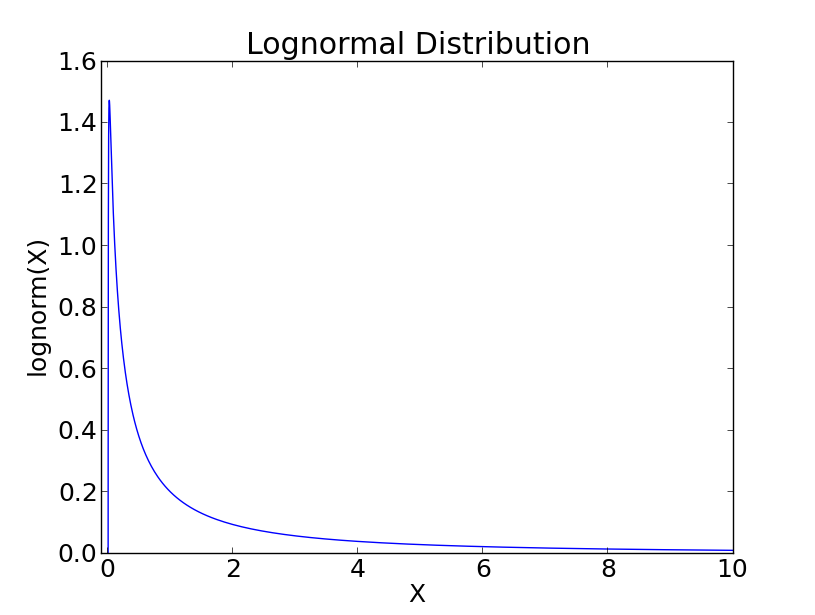
\includegraphics[width=.8\linewidth]{../Images/LogNormal_Linear.png}
  \caption{Plotted against a linear abscissa.}
  \label{fig:Lognormal_Sub1}
\end{subfigure}%
\begin{subfigure}{.5\textwidth}
  \centering
  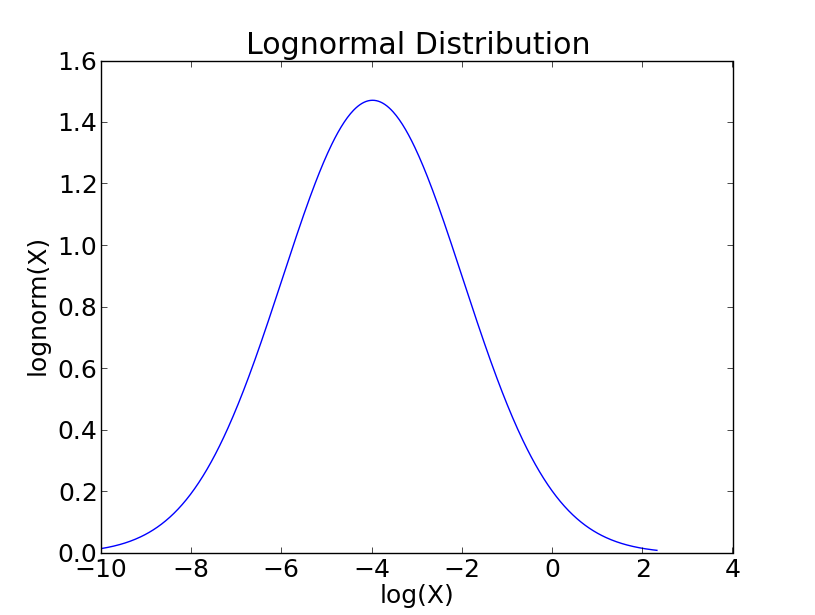
\includegraphics[width=.8\linewidth]{../Images/LogNormal_Logarithmic.png}
  \caption{Plotted against a logarithmic abscissa.}
  \label{fig:Lognormal_Sub2}
\end{subfigure}
\caption{Lognormal distribution}
\label{fig:lognormal}
\end{figure}

\subsubsection{Exponential Distribution}\index{general}{distributions!exponential}

For a stochastic variable X with an \emph{exponential distribution}, the probability distribution function is:
\begin{equation}\label{eq_exponential}
f_x (x) =
  \begin{cases}
\lambda e^{- \lambda x}, & \mbox{if } x \ge 0 \\
0, & \mbox{if } x < 0
\end{cases}
\end{equation}

The exponential PDF is shown in Figure \ref{fig:exponential}
\begin{figure}
  \centering
  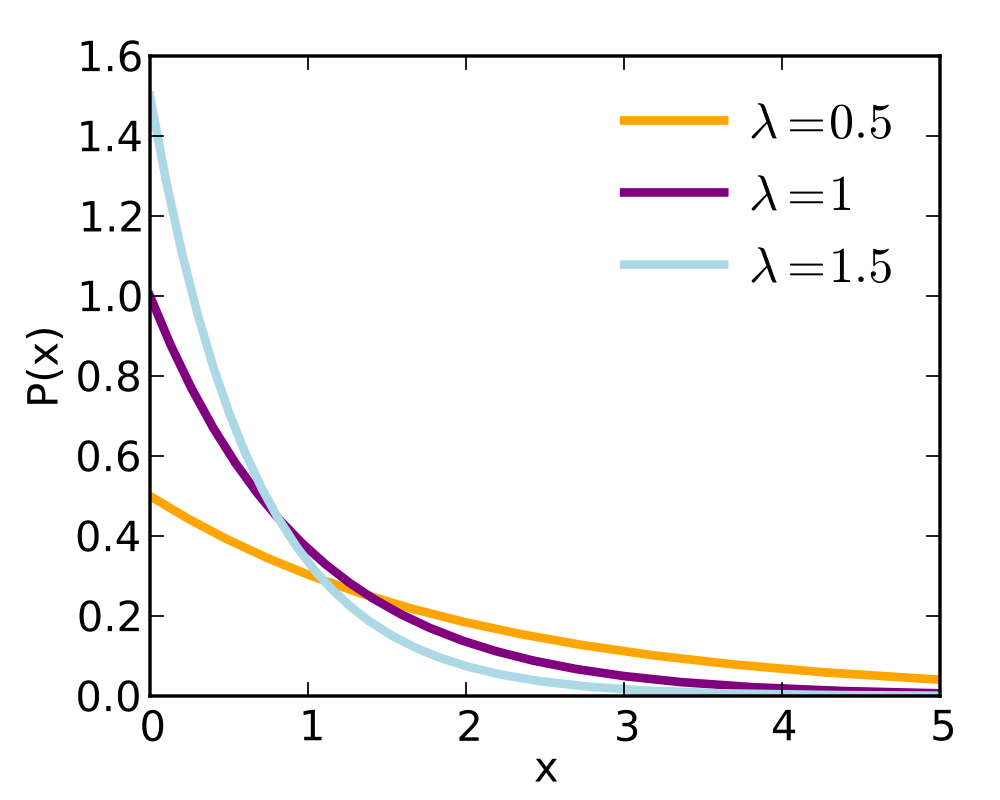
\includegraphics[width=0.5\textwidth]{../Images/Exponential_pdf.png}\\
  \caption{Exponential Distribution}\label{fig:exponential}
\end{figure}


\subsubsection{Uniform Distribution}\index{general}{distributions!uniform}

This is a simple one: an even probability for all data values (Figure \ref{fig:uniform}). Not very common for real data.

\begin{figure}
  \centering
  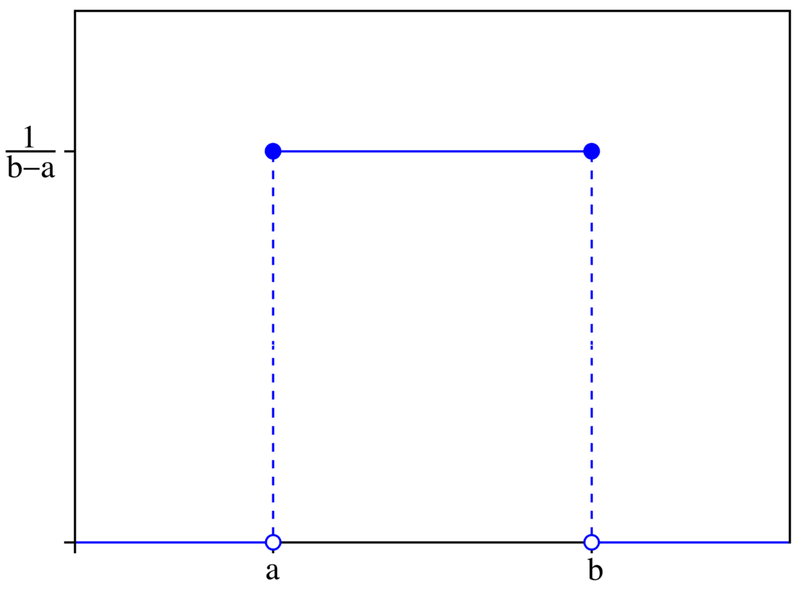
\includegraphics[width=0.5\textwidth]{../Images/Uniform_Distribution_PDF.png}\\
  \caption{Uniform Distribution} \label{fig:uniform}
\end{figure}

\subsubsection{ Programs: Continuous Distribution Functions }
%\lstinputlisting[label=py:dist_continuous,caption=dist_continuous.py, language=Python]{../Code/dist_continuous.py}
\lstinputlisting[label=py:continuous,caption=Continuous,language=Python]{../Code/dist_continuous.py}
\index{python}{distContinuous}

\subsection{Discrete Distributions}\index{general}{distributions!discrete}

While the functions describing continuous distributions are referred to as \emph{probability distribution functions}, discrete distributions are described by \emph{probability mass functions}.

\subsubsection{Binomial Distribution}\index{general}{distributions!binomial}
The Binomial is associated with the question "Out of a given number of trials, how many will succeed?" Some example questions that are modeled with a Binomial distribution are:
\begin{itemize}
  \item Out of ten tosses, how many times will this coin land ''heads''?
  \item From the children born in a given hospital on a given day, how many of them will be girls?
  \item How many students in a given classroom will have green eyes?
  \item How many mosquitos, out of a swarm, will die when sprayed with insecticide?
\end{itemize}

  We conduct $n$ repeated experiments where the probability of success is given by the parameter $p$ and add up the number of successes. This number of successes is represented by the random variable $X$.  The value of $X$ is then between 0 and $n$.

When a random variable X has a Binomial Distribution with parameters $p$ and $n$ we write it as $\,X \sim Bin(n,p)$ or $\,X \sim B(n,p)$ and the probability mass function is given at $X=k$ by the equation:

\begin{equation}
    P\left[X = k\right] = \begin{cases} {n \choose k} p^k \left(1-p\right)^{n-k}\ & 0 \le k \le n \\ 0 & \mbox{otherwise} \end{cases} \quad 0 \leq p \leq 1, \quad n \in \mathbb{N}
\end{equation}

where ${n \choose k}={n! \over k!(n-k)!}$

\begin{figure}
  \centering
  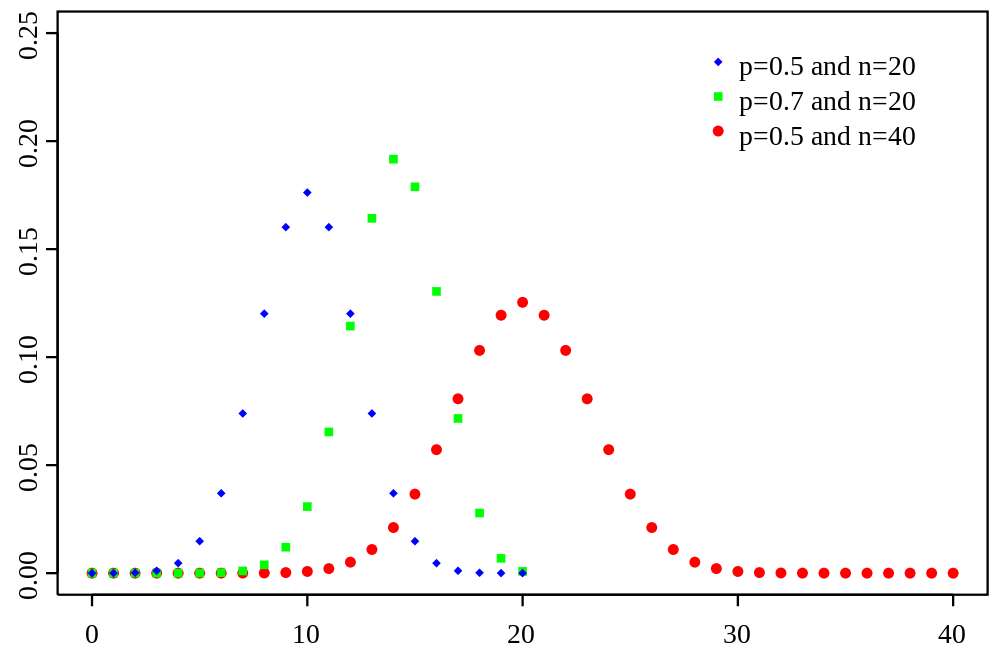
\includegraphics[width=0.75\textwidth]{../Images/Binomial_distribution_pmf.png}\\
  \caption{Binomial Distribution}
\end{figure}


\subsubsection{Poisson Distribution}\index{general}{distributions!poisson}

Any French speaker will notice that "Poisson" means "fish", but really there's nothing fishy about this distribution. It's actually pretty straightforward. The name comes from the mathematician Siméon-Denis Poisson (1781-1840).

The Poisson Distribution is ''very similar'' to the Binomial Distribution. We are examining the number of times an event happens. The difference is subtle. Whereas the Binomial Distribution looks at how many times we register a success over a fixed total number of trials, the Poisson Distribution measures how many times a discrete event occurs, over a period of continuous space or time. There isn't a "total" value n. As with the previous sections, let's examine a couple of experiments or questions that might have an underlying Poisson nature.

\begin{itemize}
  \item How many pennies will I encounter on my walk home?
  \item How many children will be delivered at the hospital today?
  \item How many products will I sell after airing a new television commercial?
  \item How many mosquito bites did you get today after having sprayed with insecticide?
  \item How many defects will there be per 100 metres of rope sold?
\end{itemize}

What's a little different about this distribution is that the random variable $X$ which counts the number of events can take on \emph{any non-negative integer} value. In other words, I could walk home and find no pennies on the street. I could also find one penny. It's also possible (although unlikely, short of an armored-car exploding nearby) that I would find 10 or 100 or 10,000 pennies.

Instead of having a parameter p that represents a component probability like in the Binomial distribution, this time we have the parameter "lambda" or $\lambda$ which represents the "average or expected" number of events to happen within our experiment. The probability mass function of the Poisson is given by

\begin{equation}
  P(X=k)=\frac{e^{-\lambda}\lambda^k}{k!}
\end{equation}.


\begin{figure}
  \centering
  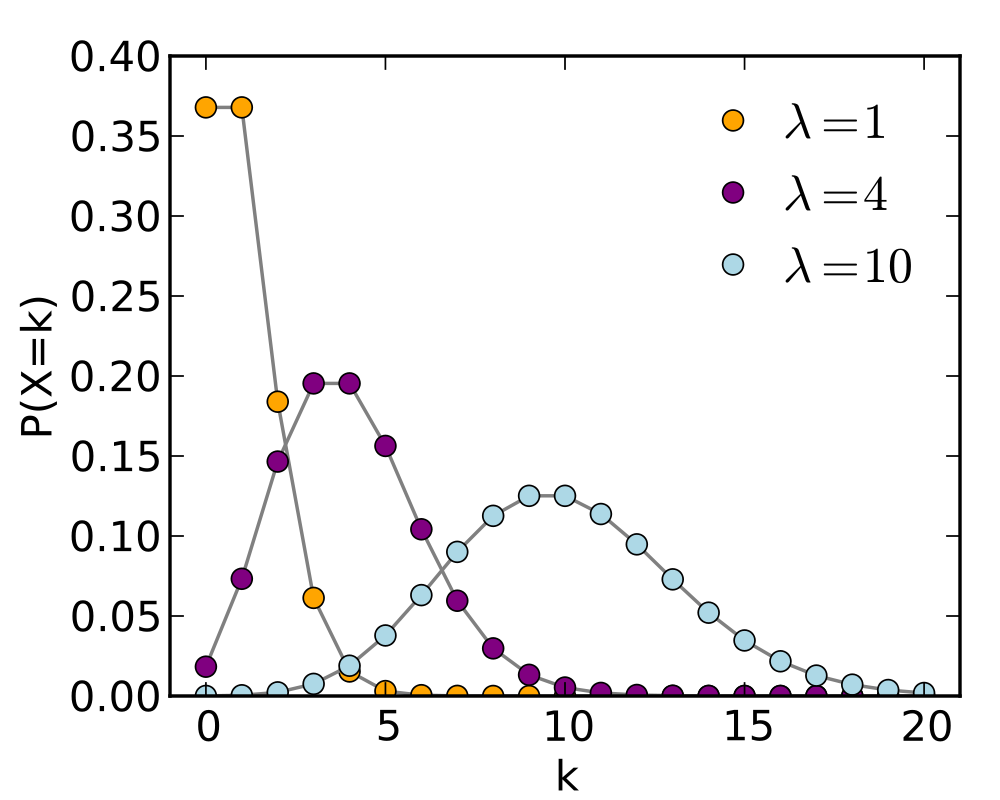
\includegraphics[width=0.5\textwidth]{../Images/Poisson_pmf.png}\\
  \caption{Poisson Distribution}
\end{figure}

\subsubsection{ Programs: Discrete Distribution Functions } \index{general}{distributions!discrete}
\lstinputlisting[label=py:discrete,caption=Discrete,language=Python]{../Code/dist_discrete.py}
\index{python}{distDiscrete}

%(Lecture 7)

\section{Data Analysis}

\subsection{Data Screening}

The first thing you have to do for your data analysis is simply \emph{look at your data}. You should check for \emph{missing data} in your data set, and \emph{outliers} which can significantly influence the result of your analysis.

\subsection{Normality Check} \index{general}{normality check} \index{general}{plots!$Q-Q$ plot}
The first way to check if your data are normally distributed, i.e. that they are linearly related to the standard normal distribution. In statistics, \emph{$Q–Q$ plots} ("Q" stands for quantile) are used for visual assessments of distributions. They are a graphical method for comparing two probability distributions by plotting their quantiles against each other. First, the set of intervals for the quantiles are chosen. A point $(x,y)$ on the plot corresponds to one of the quantiles of the second distribution (y-coordinate) plotted against the same quantile of the first distribution (x-coordinate). Thus the line is a parametric curve with the parameter which is the (number of the) interval for the quantile.

If the two distributions being compared are similar, the points in the $Q-Q$ plot will approximately lie on the line $y = x$. If the distributions are linearly related, the points in the $Q-Q$ plot will approximately lie on a line, but not necessarily on the line $y = x$ (Figure \ref{fig:qqplot}).

\begin{figure}
  \centering
  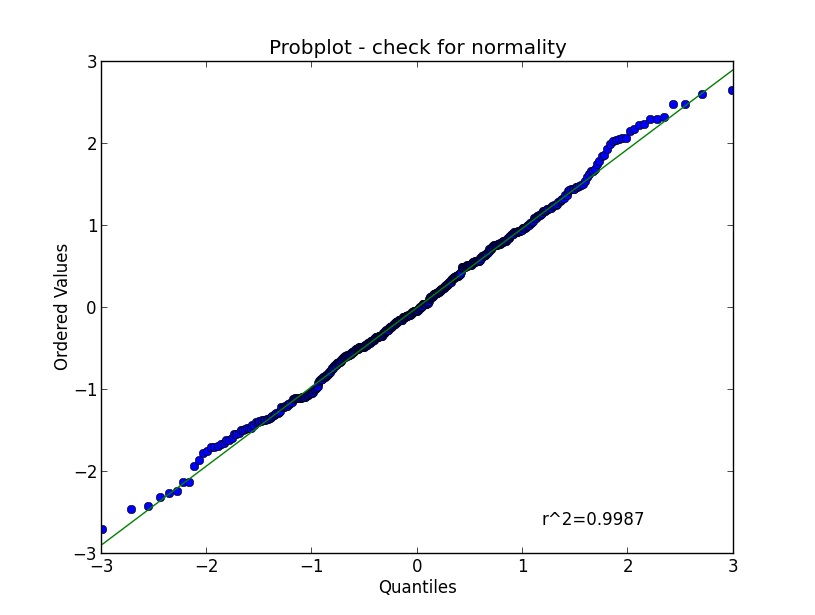
\includegraphics[width=0.75\textwidth]{../Images/ProbPlot.png}\\
  \caption{QQ-Plot, to check for normality of distribution.}\label{fig:qqplot}
\end{figure}

In addition, there are quantitative tests for normality. The test that I have encountered most frequently in recent literature is the \emph{Kolmogorov-Smirnov test}.
\footnote{see scipy.stats.kstest, example given in univariate.py}
Altman mainly uses the \emph{Shapiro-Wilk W test} \cite{altman99}, and a number of other tests are also available.

\subsection{Transformation} \index{general}{transformation}
If your data deviate significantly from a normal distribution, it is sometimes possible to make the distribution approximately normal by transforming your data. For example, data often have values that can only be positive (e.g. the size of persons), and that have  long positive tail: such data can often be made normal by applying a \emph{log transform}. This is demonstrated in Figure \ref{fig:lognormal}.

\subsection{Confidence Intervals}\index{general}{confidence interval}
Although it is common to concentrate the analysis on the p-values, it is often much more informative to report the \emph{confidence intervals} for your data. The confidence intervals are given by

\begin{equation}
  ci = mean \pm se * t_{n,\alpha}
\end{equation}

where $se$ is the standard error, and $t_{n,\alpha}$ the $t$ statistic for $n$ degrees of freedom. For the 95\% two-sided confidence intervals, for example, you have to set $\alpha=0.025$ and $\alpha=0.975$ .
